% The pointer jumping of Wyllie on the list 3, 6, 0, 5, 1, 7, 2, 4 (the tail
% 4), sec. 23.5: the ranks r and the successors s of the items after each
% round, the item 3 (the head) in violet; after 3 rounds every s is the
% tail and r is the rank. Build: make figures (in ../build).
\documentclass[border=4pt]{standalone}
\usepackage[T1]{fontenc}
\usepackage{lmodern}
\usepackage{amsmath,amssymb}
\usepackage{tikz}
\usepackage{lamalunga}
% tikz-ads.tex: the TikZ styles shared by the figures of the memory of the
% manual, \input by each standalone figure: a cell of a vector (cell), the
% cell that an operation touches (touched), a free cell (free), a node of a
% linked structure (node), the labels of indices (index) and of variables
% (var), a pointer (ptr), and \cells and \indices to draw a row of cells.
\usetikzlibrary{arrows.meta,positioning,calc,fit,shapes.multipart}
\definecolor{adsTouched}{RGB}{214,196,236}
\definecolor{adsFree}{RGB}{236,236,236}
\tikzset{
  ads/.style={>={Stealth[length=2mm]},font=\small,
              every node/.append style={inner sep=0pt}},
  cell/.style={draw,minimum width=7mm,minimum height=7mm,
               font=\small\ttfamily,outer sep=0pt},
  touched/.style={cell,fill=adsTouched},
  free/.style={cell,fill=adsFree,text=black!45},
  node/.style={draw,rounded corners=1pt,minimum width=8mm,
               minimum height=6mm,font=\small\ttfamily},
  index/.style={font=\scriptsize\ttfamily,text=black!60},
  var/.style={font=\small\itshape},
  ptr/.style={->,thick}
}
% \cells{name}{x,y}{list}: a row of cells, the first at (x,y), named
% name-0, name-1, ...; each item is text/style, the style one of cell,
% touched and free (e.g., {a/cell,e/touched,/free})
\newcommand{\cells}[3]{%
  \foreach \v/\s [count=\i from 0] in {#3}
    \node[\s] (#1-\i) at ($(#2)+(\i*7mm,0)$) {\v};}
% \indices{name}{n}: the indices 0 .. n-1 under the cells of name
\newcommand{\indices}[2]{%
  \foreach \i in {0,...,\numexpr#2-1\relax}
    \node[index,below=1.2mm of #1-\i] {\i};}

\begin{document}
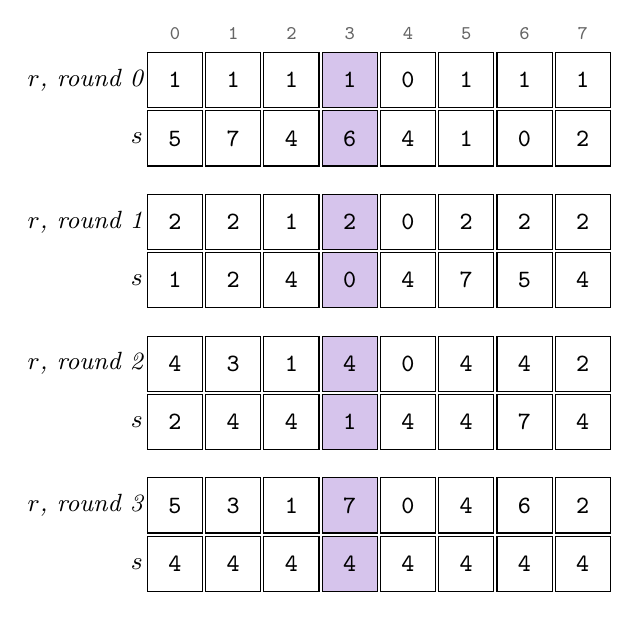
\begin{tikzpicture}[ads]
  \node[var,anchor=east] at (-4mm,0mm) {$r$, round 0};
  \node[cell] (r0-0) at (0mm,0mm) {1};
  \node[cell] (r0-1) at (7.4mm,0mm) {1};
  \node[cell] (r0-2) at (14.8mm,0mm) {1};
  \node[touched] (r0-3) at (22.2mm,0mm) {1};
  \node[cell] (r0-4) at (29.6mm,0mm) {0};
  \node[cell] (r0-5) at (37mm,0mm) {1};
  \node[cell] (r0-6) at (44.4mm,0mm) {1};
  \node[cell] (r0-7) at (51.8mm,0mm) {1};
  \node[var,anchor=east] at (-4mm,-7.4mm) {$s$};
  \node[cell] (s0-0) at (0mm,-7.4mm) {5};
  \node[cell] (s0-1) at (7.4mm,-7.4mm) {7};
  \node[cell] (s0-2) at (14.8mm,-7.4mm) {4};
  \node[touched] (s0-3) at (22.2mm,-7.4mm) {6};
  \node[cell] (s0-4) at (29.6mm,-7.4mm) {4};
  \node[cell] (s0-5) at (37mm,-7.4mm) {1};
  \node[cell] (s0-6) at (44.4mm,-7.4mm) {0};
  \node[cell] (s0-7) at (51.8mm,-7.4mm) {2};
  \node[var,anchor=east] at (-4mm,-18mm) {$r$, round 1};
  \node[cell] (r1-0) at (0mm,-18mm) {2};
  \node[cell] (r1-1) at (7.4mm,-18mm) {2};
  \node[cell] (r1-2) at (14.8mm,-18mm) {1};
  \node[touched] (r1-3) at (22.2mm,-18mm) {2};
  \node[cell] (r1-4) at (29.6mm,-18mm) {0};
  \node[cell] (r1-5) at (37mm,-18mm) {2};
  \node[cell] (r1-6) at (44.4mm,-18mm) {2};
  \node[cell] (r1-7) at (51.8mm,-18mm) {2};
  \node[var,anchor=east] at (-4mm,-25.4mm) {$s$};
  \node[cell] (s1-0) at (0mm,-25.4mm) {1};
  \node[cell] (s1-1) at (7.4mm,-25.4mm) {2};
  \node[cell] (s1-2) at (14.8mm,-25.4mm) {4};
  \node[touched] (s1-3) at (22.2mm,-25.4mm) {0};
  \node[cell] (s1-4) at (29.6mm,-25.4mm) {4};
  \node[cell] (s1-5) at (37mm,-25.4mm) {7};
  \node[cell] (s1-6) at (44.4mm,-25.4mm) {5};
  \node[cell] (s1-7) at (51.8mm,-25.4mm) {4};
  \node[var,anchor=east] at (-4mm,-36mm) {$r$, round 2};
  \node[cell] (r2-0) at (0mm,-36mm) {4};
  \node[cell] (r2-1) at (7.4mm,-36mm) {3};
  \node[cell] (r2-2) at (14.8mm,-36mm) {1};
  \node[touched] (r2-3) at (22.2mm,-36mm) {4};
  \node[cell] (r2-4) at (29.6mm,-36mm) {0};
  \node[cell] (r2-5) at (37mm,-36mm) {4};
  \node[cell] (r2-6) at (44.4mm,-36mm) {4};
  \node[cell] (r2-7) at (51.8mm,-36mm) {2};
  \node[var,anchor=east] at (-4mm,-43.4mm) {$s$};
  \node[cell] (s2-0) at (0mm,-43.4mm) {2};
  \node[cell] (s2-1) at (7.4mm,-43.4mm) {4};
  \node[cell] (s2-2) at (14.8mm,-43.4mm) {4};
  \node[touched] (s2-3) at (22.2mm,-43.4mm) {1};
  \node[cell] (s2-4) at (29.6mm,-43.4mm) {4};
  \node[cell] (s2-5) at (37mm,-43.4mm) {4};
  \node[cell] (s2-6) at (44.4mm,-43.4mm) {7};
  \node[cell] (s2-7) at (51.8mm,-43.4mm) {4};
  \node[var,anchor=east] at (-4mm,-54mm) {$r$, round 3};
  \node[cell] (r3-0) at (0mm,-54mm) {5};
  \node[cell] (r3-1) at (7.4mm,-54mm) {3};
  \node[cell] (r3-2) at (14.8mm,-54mm) {1};
  \node[touched] (r3-3) at (22.2mm,-54mm) {7};
  \node[cell] (r3-4) at (29.6mm,-54mm) {0};
  \node[cell] (r3-5) at (37mm,-54mm) {4};
  \node[cell] (r3-6) at (44.4mm,-54mm) {6};
  \node[cell] (r3-7) at (51.8mm,-54mm) {2};
  \node[var,anchor=east] at (-4mm,-61.4mm) {$s$};
  \node[cell] (s3-0) at (0mm,-61.4mm) {4};
  \node[cell] (s3-1) at (7.4mm,-61.4mm) {4};
  \node[cell] (s3-2) at (14.8mm,-61.4mm) {4};
  \node[touched] (s3-3) at (22.2mm,-61.4mm) {4};
  \node[cell] (s3-4) at (29.6mm,-61.4mm) {4};
  \node[cell] (s3-5) at (37mm,-61.4mm) {4};
  \node[cell] (s3-6) at (44.4mm,-61.4mm) {4};
  \node[cell] (s3-7) at (51.8mm,-61.4mm) {4};
  \foreach \i in {0,...,7} \node[index,above=1.6mm of r0-\i] {\i};
\end{tikzpicture}
\end{document}
